% \documentclass[11pt]{article}
% \usepackage{../lecnotes}
\chapter{Tries}
\label{ch:tries}

\newcommand{\lecnum}{22}
%\newcommand{\lectitle}{Tries}
\newcommand{\lecturer}{Thomas Cortina, Frank Pfenning, Rob Simmons,
  Penny Anderson}

\chapterTAGS{application, linked-list, search, trie}
\begin{document}
\maketitle

\noindent
In the data structures implementing associative arrays so far, we have
needed either an equality operation and a hash function, or a
comparison operator with a total order on keys.  Similarly, our
sorting algorithms just used a total order on keys and worked by
comparisons of keys.  We obtain a different class of representations
and algorithms if we analyze the structure of keys and decompose them.
In this lecture we explore \emph{tries}, an example from this class of
data structures.  The asymptotic complexity we obtain has a different
nature from data structures based on comparisons, depending on the
structure of the key rather than the number of elements stored in
the data structure.

\section{The Boggle Word Game}
\TAGS{application, search}

The Boggle word game is played on an $n \times n$ grid (usually $4
\times 4$ or $5 \times 5$).  We have $n \times n$ dice that have letters on
all 6 sides and which are shaken so that they randomly settle into the
grid.  At that point we have an $n \times n$ grid filled with letters.
Now the goal is to find as many words as possible in this grid within
a specified time limit.  To construct a word we can start at an
arbitrary position and use any of the 8 adjacent letters as the second
letter.  From there we can again pick any adjacent letter as the third
letter in the word, and so on.  We may not reuse any particular
place in the grid in the same word, but they may be in common for different
words.  For example, in the grid
\[\begin{tabular}{|c|c|c|c|}
  \hline
  E & F & R & A \\[0.6ex] \hline
  H & G & D & R \\[0.6ex] \hline
  P & S & N & A \\[0.6ex] \hline
  E & E & B & E \\[0.6ex] \hline
\end{tabular}\]
we have the words \textsf{SEE}, \textsf{SEEP}, and \textsf{BEARDS},
but not \textsf{SEES}.  Scoring assigns points according to the lengths
of the words found, where longer words score higher.

One simple possibility for implementing this game is to systematically
search for potential words and then look them up in a dictionary,
perhaps stored as a sorted word list, some kind of binary search tree,
or a hash table.  The problem is that there are too many potential
words on the grid, so we want to consider prefixes and abort the
search when a prefix does not start a word.  For example, if we start
in the upper left-hand corner and try horizontally first, then
\textsf{EF} is a prefix for a number of words, but \textsf{EFR},
\textsf{EFD}, \textsf{EFG}, \textsf{EFH} are not and we can abandon
our search quickly.  A few more possibilities reveal that no word with
3 letters or more in the above grid starts in the upper left-hand
corner.

Because a dictionary is sorted alphabetically, by prefix, we may
be able to use a sorted array effectively in order for the computer to
play Boggle and quickly determine all possible words on a grid.  But
we may still look for potentially more efficient data structures which
take into account that we are searching for words that are
constructed by incrementally extending the prefix.

\section{Multi-Way Tries}
\TAGS{trie}

One possibility is to use a \emph{multi-way trie}, where each node has
a potential child for each letter in the alphabet.  Consider the word
\textsf{SEE}.  We start at the root and follow the link labeled
\textsf{S}, which gets us to a node on the second level in the tree.
This tree indexes all words with first character \textsf{S}.  From
here we follow the link labeled \textsf{E}, which gets us to a node
indexing all words that start with \textsf{SE}.  After one more step
we are at \textsf{SEE}.  At this point we cannot be sure if this is a
complete word or just a prefix for words stored in it.  In order to
record this, we can either store a Boolean (\lstinline'true' if the current
prefix is a complete word) or terminate the word with a special
character that cannot appear in the word itself.

Below is an example of a multi-way trie indexing the three words
\textsf{BE}, \textsf{BEE}, and \textsf{BACCALAUREATE}.
\begin{center}
  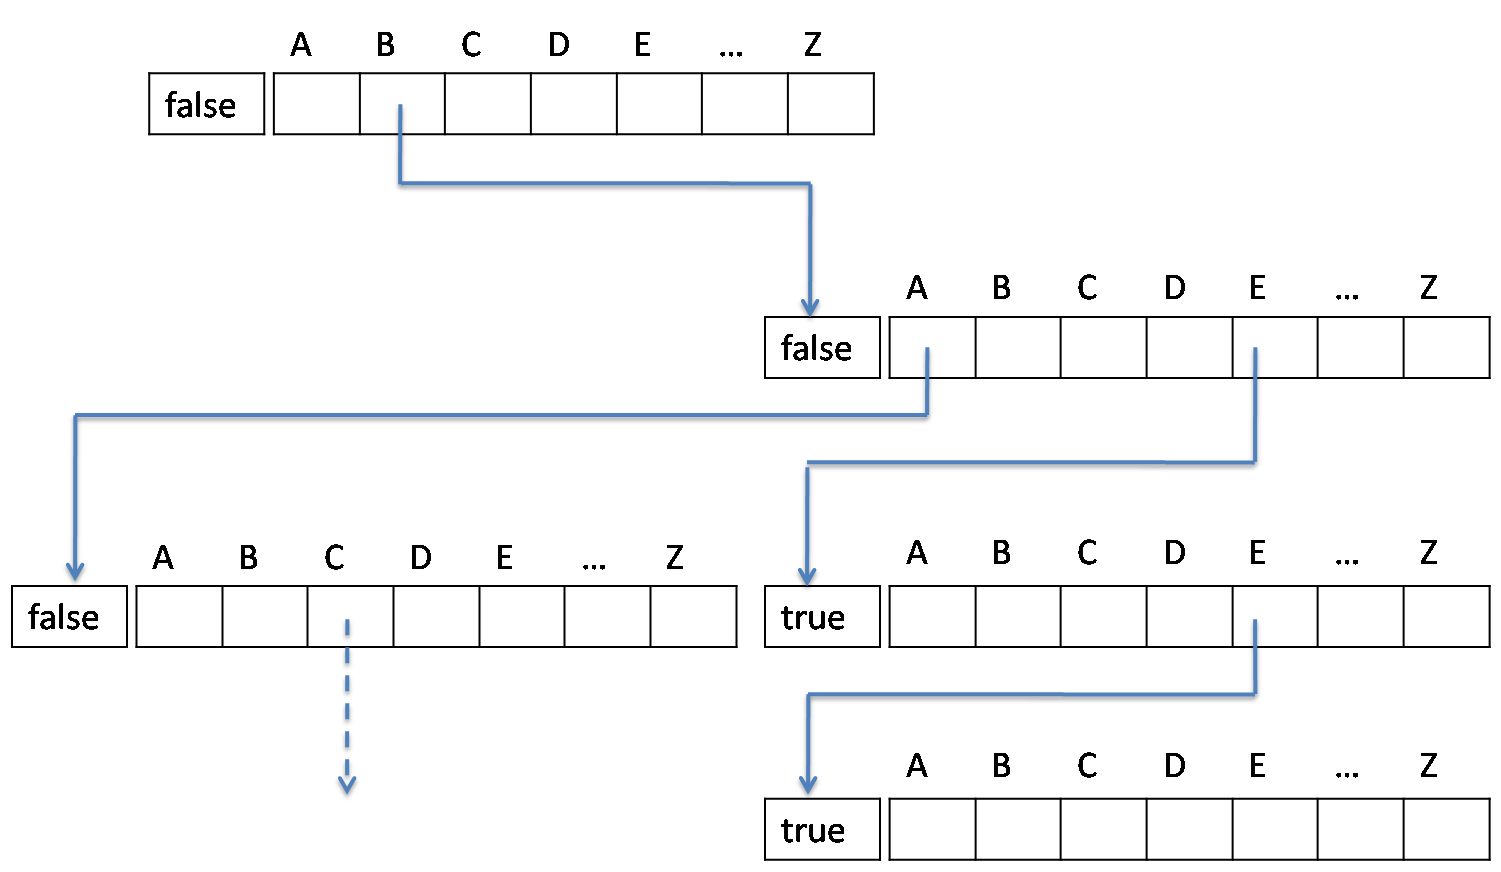
\includegraphics[width=0.99\textwidth]{\img/tries1.png}
\end{center}
While the paths to finding each word are quite short, including one
more node than characters in the word, the data structure consumes a
lot of space, because there are a lot of nearly empty arrays.

An interesting property is that the lookup time for a word is $O(k)$,
where $k$ is the number of characters in the word.  This is
independent of how many words are stored in the data structure!
Contrast this with, say, balanced binary search trees where the search
time is $O(\mathrm{log}(n))$, where $n$ is the number of words stored.
For the latter analysis we assumed that key comparisons were constant
time, which is not really true because the keys (which are strings)
have to be compared character by character.  So each comparison, while
searching through a binary search tree, might take up to $O(k)$
individual character comparisons, which would make it $O(k *
\mathrm{log}(n))$ in the worst case.  Compare that with $O(k)$ for a
trie.

On the other hand, the wasted space of the multi-way trie with an
array at each node costs time in practice.  This is not only because
this memory must be allocated, but because on modern architectures the
so-called \emph{memory hierarchy} means that accesses to memory cells
close to each other will be much faster than accessing distant cells.
You will learn more about this in 15-213 \emph{Computer Systems}.

\section{Binary Tries}
\TAGS{trie}

The idea of the multi-way trie is quite robust, and there are useful
special cases.  One of these if we want to represent sets of numbers.
In that case we can decompose the binary representation of numbers bit
by bit in order to index data stored in the trie.  We could start with
the most significant or least significant bit, depending on the kind
of numbers we expect.  In this case every node would have at most two
successors, one for $0$ and one for $1$.  This does not waste nearly
as much space and can be efficient for many purposes.

\section{Linked Lists}
\TAGS{linked-list, trie}

For the particular application we have in mind, namely searching
for words on a grid of letters, we could either use multiway tries
directly (wasting space) or use binary tries (wasting time and space,
because each character is decomposed into individual bits).

A compromise solution is replacing the array (which may end up mostly
empty) with a linked list. This gives us two fundamentally different
uses of pointers. Child pointers (drawn in blue) correspond to forward
movement through the string. The next pointers of the linked list
(drawn in red), on the other hand, connect what used to be parts of
the same array list.

In this representation, it also becomes natural to have the Boolean
``end of word'' flag stored with the final character, rather than one
step below the final character like we did above. (This means it's no
longer possible to store the empty string, however.) The tree above,
containing \textsf{BACCALAUREATE}, \textsf{BE}, and \textsf{BEE}, now
looks like this:
\begin{center}
  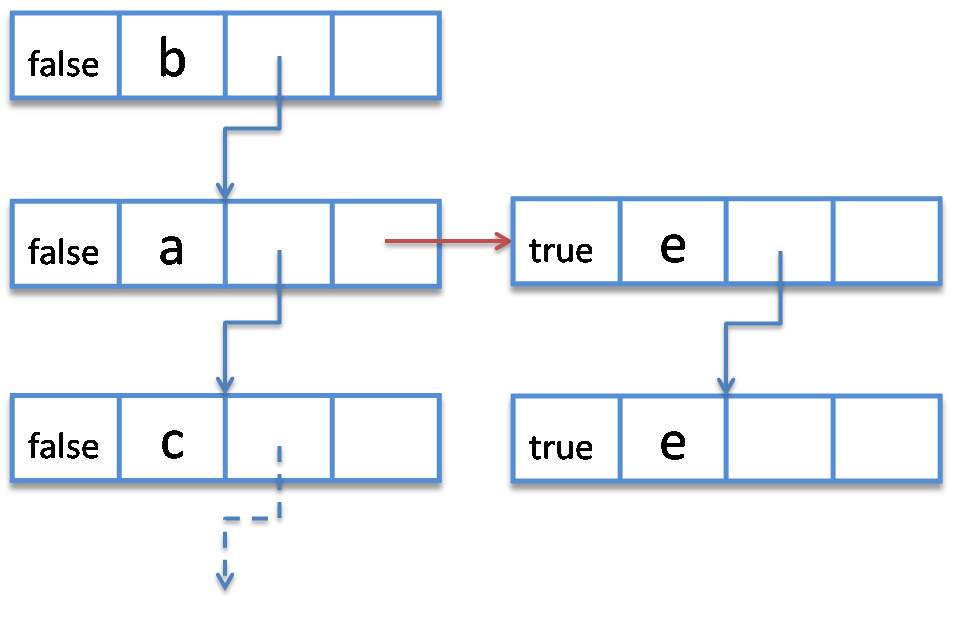
\includegraphics[width=0.6\textwidth]{\img/tries3.png}
\end{center}
If we add \textsf{OR} and \textsf{BED}, the result looks like this:
\begin{center}
  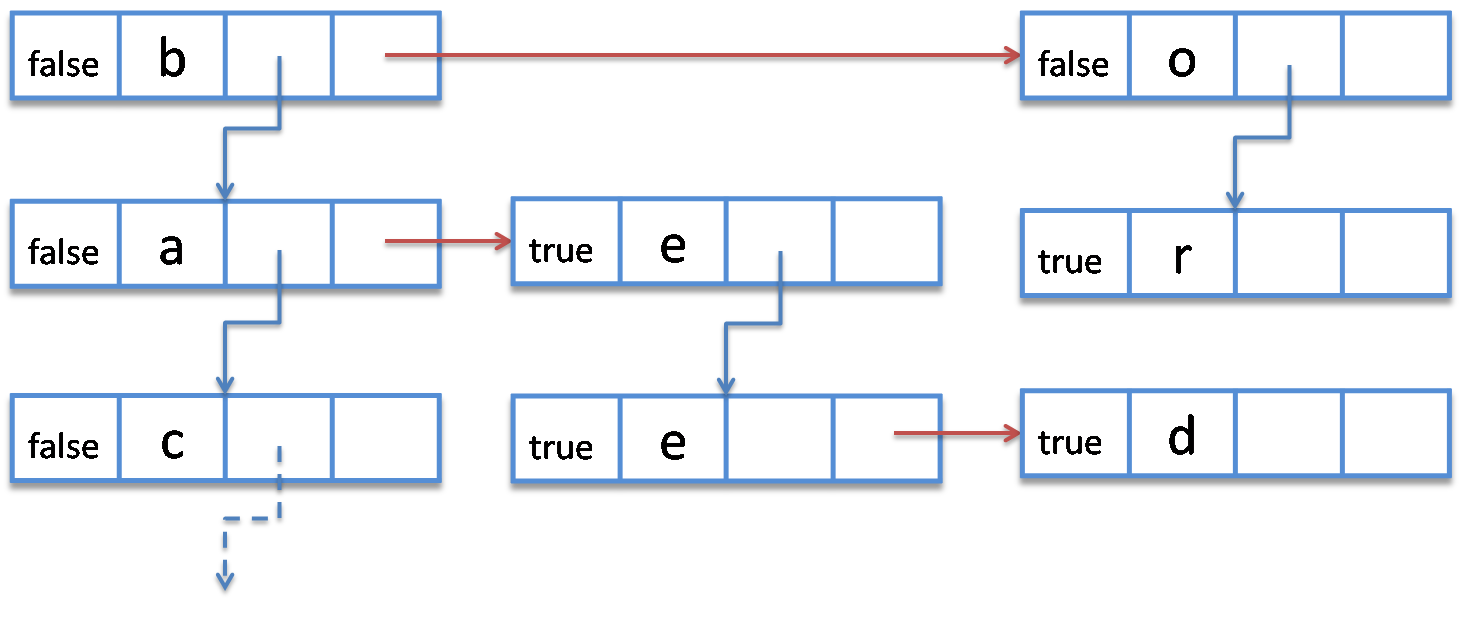
\includegraphics[width=0.9\textwidth]{\img/tries4.png}
\end{center}

For lookup, we have to make at most 26 comparisons between each
character in the input string and the characters stored in the tree.
Therefore search time is $O(26*k) = O(k)$, where $k$ is the length of
the string.  Insertion has the same asymptotic complexity bound.  Note
that this still does not change with the number of strings, only with its
length.


\section{Ternary Search Tries}
\TAGS{trie}

It should be apparent that we could get some performance gains over
this linked list solution if we kept the linked lists sorted. This is
an idea that allows us to motivate a more suitable data structure, a
\emph{ternary search trie} (TST) which combines ideas from binary
search trees with tries.  Roughly, at each node in a trie we store a
binary search tree with characters as keys.  The entries are pointers
to the subtries.

More precisely, at each node we store a character $c$ and three
pointers.  The left subtree stores all words starting with characters
alphabetically less than $c$.  The right subtree stores all words
starting with characters alphabetically greater than $c$ and the
middle stores a subtrie with all words starting with $c$, from the
second character on.  The middle children work exactly like the child
pointers from our linked list implementation. The left and right
pointers work like the next pointers from the linked list version, and
are correspondingly drawn in red in the diagram below, which contains
the words \textsf{BE}, \textsf{BED}, \textsf{BEE},
\textsf{BACCALAUREATE}, and \textsf{OR}. In this diagram, we represent
the flag for ``end of word'' using the presence or absence of an X.

\begin{center}
  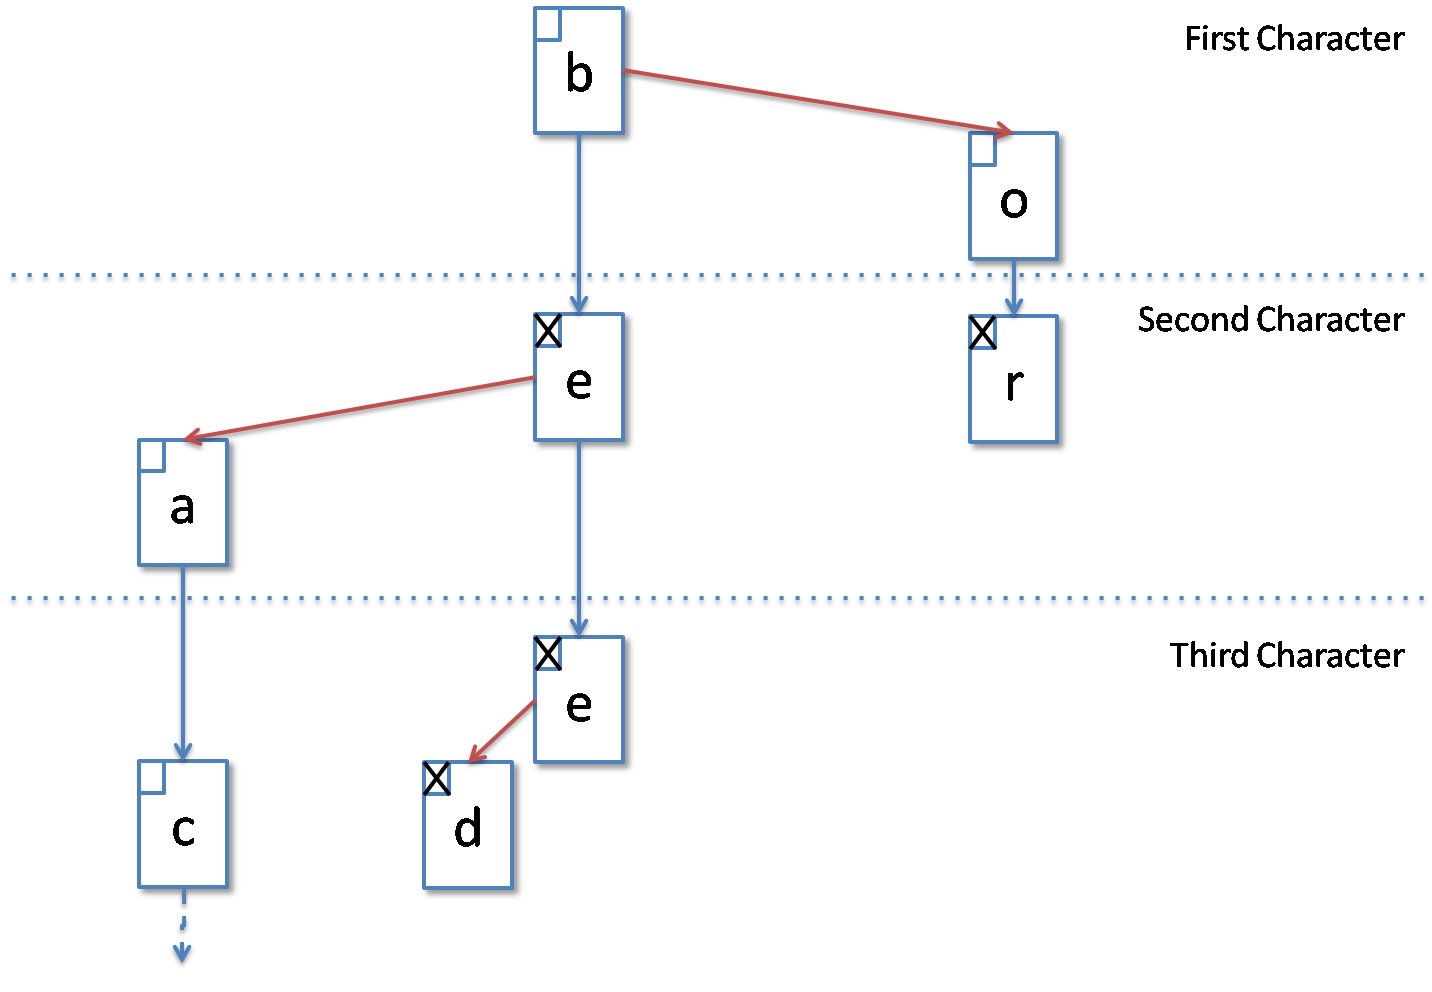
\includegraphics[width=0.9\textwidth]{\img/tries5.png}
\end{center}


We have not discussed any strategy for balancing TSTs. However, in the
worst case (a completely unbalanced tree) we end up with something
similar to the linked list implementation and we have to make at most
26 comparisons between each character in the input string and the
characters stored in the tree.  Therefore search time is $O(26*k) =
O(k)$, where $k$ is the length of the string.  Even when the embedded
trees are perfectly balanced, the constant factor decreases, but not
the asymptotic complexity because $O(\mathrm{log}(26)*k) = O(k)$.

\section*{Exercises}

\begin{exercise}
  Implement the game of Boggle as sketched in this lecture.
  Make sure to pick the letters according to the distribution
  of their occurrence in the English language.  You might
  use the Scrabble dictionary itself, for example, to calculate
  the relative frequency of the letters.

  If you are ambitious, try to design a simple textual interface
  to print a random grid and then input words from the human
  player and show the words missed by the player.
\end{exercise}

\begin{exercise}
  Modify the implementation TSTs so it can store, for each word, the
  number of occurrences of that word in a book that is read word by
  word.
\end{exercise}

\begin{exercise}
  Modify the implementation of search in TSTs so it can process
  a star (\lstinline"'*'") character in the search string.  It can
  match any number of characters for words stored in the trie.
  This matching is done by adding all matching string to a queue
  that is an input argument to the generalized search function.

  For example, after we insert \textsf{BE}, \textsf{BED}, and
  \textsf{BACCALAUREATE}, the string \lstinline'"BE*"' matches the first
  two words, and \lstinline'"*A*"' matches the only the third, in three
  different ways.  The search string \lstinline'"*"' should match the
  entire set of words stored in the trie and produce them in
  alphabetical order.  You should decide if the different ways to
  match a search string should show up multiple times in the result
  queue or just one.
\end{exercise}

\begin{exercise}
Modify TSTs to use a special non-alphabetic character (either period
\lstinline"'.'" or the nil character \lstinline"'\0'"), which is shown as a
small filled circle in the diagram, to represent the end of the word.
\begin{center}
  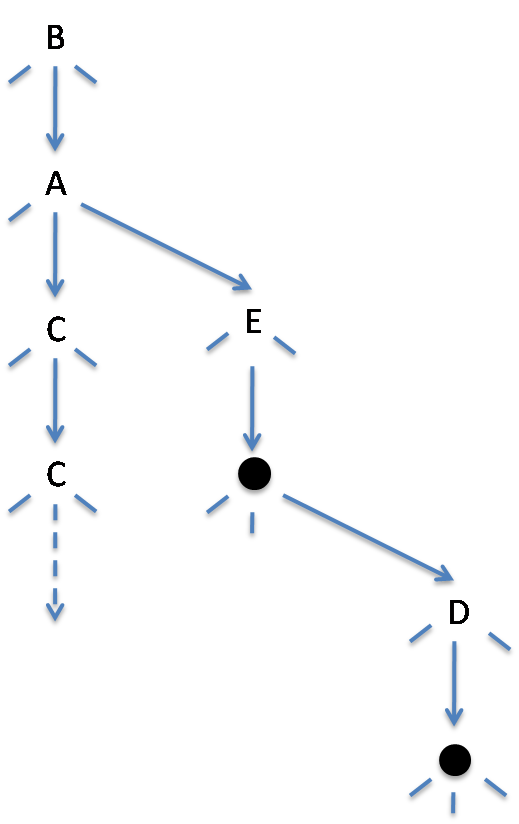
\includegraphics[width=0.4\textwidth]{\img/tries2.png}
\end{center}
\end{exercise}

\begin{exercise}
Using this modified TST implementation from the question above,
allow repeated searching of prefixes with the following interface:
\begin{lstlisting}[language=c]
/* Prefix search interface */
typedef struct trie_node tnode;
tnode *trie_root(trie TR);
tnode *tnode_lookup_prefix(tnode *T, char *s); /* i < strlen(s) */
elem tnode_elem(tnode *T);
\end{lstlisting}
The \lstinline'tnode' pointer returned by \lstinline'trie_root' or
\lstinline'tnode_lookup_prefix' should be a pointer to the root of a TST,
and \lstinline'tnode_elem' will look for the the special character
\lstinline"'.'" or \lstinline"'\0'" by following \lstinline'left' and \lstinline'right'
pointers and return any data stored at that special node.
\end{exercise}

\begin{exercise}
Consider other implementations of the interface above that allow
repeated searching of prefixes.
\end{exercise}

\begin{exercise}
  Implement sets of 32-bit integers as binary tries, including
  functions for testing set membership, intersection, union,
  and set difference.
\end{exercise}

\begin{exercise}
  Compare your implementation if integer sets with an implementation
  as binary search trees (assuming random insertion to avoid the
  complexities of rebalancing).  Which operations on which kinds of
  sets would be more efficient in one representation than the other?
\end{exercise}


\end{document}

% \begin{comment}
% \section{Specifying an Interface}

% Specifying an interface for tries is tricky.  If we want to just use
% tries as dictionaries, then we can store arbitrary elements, but we
% commit to strings as keys. In that sense our interface is not very
% abstract, but well-suited to our application. (To relate this to our
% discussion above, an X in the diagram above can represent the presence
% or absence of an element rather than a \lstinline'bool' flag.)

% \begin{lstlisting}[language=c]
% typedef struct trie_header *trie;

% trie trie_new();
% elem trie_lookup(trie TR, char *s);
% void trie_insert(trie TR, char *s, elem e);
% void trie_free(trie TR);
% \end{lstlisting}

% The interface above is unable to handle freeing the data encoded in a
% trie. We discussed a client interface function \lstinline'elem_free' when
% we ported binary search trees to C, but here we treat it as the
% client's responsibility to track and free their elements. If we
% \lstinline'typedef' the type \lstinline'elem' to be a void pointer, we now have
% a data structure without generic keys (keys are defined to be strings)
% but with generic values. By casting into and out of \lstinline'void*', we
% can store different values in the trie without duplicating the algorithm and data structure code the way we
% did in Claclab.

% \section{Adapting the interface}

% However, it turns out we oversimplified.  While the interface works
% well to use the trie as a kind of dictionary, it does not work well
% for our boggle application since we cannot tell if a string is a valid
% prefix of a complete word or not.

% If we want to be able to search for valid prefixes in tries, not just
% complete words, one option is to expose to the user a little bit of
% what the internal structure of a trie looks like. The function
% \lstinline'trie_lookup_prefix' returns a sub-trie (or \lstinline'NULL' if the
% prefix is not in the trie) and the function \lstinline'tnode_elem' checks
% to see if there is data (a checkmark) stored in that location in the
% trie.

% \begin{lstlisting}[language=c]
% typedef struct trie_node tnode;
% tnode *trie_lookup_prefix(trie T, char *s);
% elem tnode_elem(tnode *T);                  /* T != NULL */
% \end{lstlisting}

% Exposing more of our interface always comes with a cost, because we
% may be less able to change our internal representation of tries once
% we have exposed a richer interface. However, if our goal is to use
% tries to play Boggle, some interface that checks prefixes is
% absolutely necessary.

% \section{Checking Invariants}

% The declaration of the types is completely straightforward.

% \begin{lstlisting}[language=c]
% typedef struct tst_node tst;
% struct tst_node {
%   char c;           /* discriminating character */
%   elem data;        /* possible data element (void pointer) */
%   tst *left;        /* left child in bst */
%   tst *middle;      /* subtrie following c */
%   tst *right;       /* right child in bst */
% };

% struct trie_header {
%   tst *root;
% };
% \end{lstlisting}

% To check that a trie is valid we use two mutually recursive functions.
% One checks the order invariant for the binary search trees embedded in
% the trie, the other checks the correctness of the subtries.  For
% mutually recursive functions we need to forward-declare the function
% which comes textually second in the file so that type checking by the
% compiler can be done in order.

% \begin{lstlisting}[language=c]
% bool is_tst(tst *T, int lower, int upper);
% bool is_tst_root(tst *T);

% bool is_tst(tst *T, int lower, int upper) {
%   if (T == NULL) return true;
%   if (!(lower < T->c && T->c < upper)) return false;
%   if (!(is_tst(T->left, lower, T->c))) return false;
%   if (!(is_tst_root(T->middle))) return false;
%   if (!(is_tst(T->right, T->c, upper))) return false;
%   if (T->middle == NULL && T->data == NULL) return false;
%   return true;
% }

% bool is_tst_root(tst *T) {
%   return is_tst(T, 0, ((int)CHAR_MAX)+1);
% }
% \end{lstlisting}
% It only makes sense to add one to \lstinline'CHAR_MAX' because \lstinline'int'
% is a bigger type than \lstinline'char'. \lstinline'0' and \lstinline'CHAR_MAX+1'
% essentially function as $-\infty$ and $+\infty$ for checking the
% intervals of a binary search tree with strictly positive character
% values as keys.

% \section{Implementing Lookup on TSTs}

% Implementing lookup is just a direct combination of traversing a trie
% and searching through binary search trees.  We pass a trie $T$, a
% string $s$ and an index $i$ which should be a valid string index so
% that we can compare \lstinline's[i]' to the node's character.

% If $T$ is null, the word is not stored in the trie and we return
% \lstinline'NULL'.  On the other hand, if we are at the end of the string
% (\lstinline"s[i+1] = '\0'") we return the stored data.  Otherwise, we
% continue lookup in the left, middle, or right subtree as appropriate.
% Important for the last case: if the string character \lstinline's[i]' is equal
% to the character stored at the node, then we look for the
% \emph{remainder} of the word in the middle subtrie.  This is
% implemented by passing $i+1$ to the subtrie.


% \begin{lstlisting}[language=c]
% tnode *tnode_lookup(tnode *T, char *s, size_t i)
% {
%   REQUIRES(is_tst_root(T));
%   REQUIRES(s != NULL);
%   REQUIRES(i < strlen(s));

%   if (T == NULL) return NULL;
%   if (s[i] < T->c) return tnode_lookup(T->left, s, i);
%   if (s[i] > T->c) return tnode_lookup(T->right, s, i);
%   ASSERT(s[i] == T->c);
%   if (s[i+1] == '\0') return T;

%   return tnode_lookup(T->middle, s, i+1);
% }
% \end{lstlisting}
% This function can then be used to implement several interface functions:
% \begin{lstlisting}[language=c]
% tnode *trie_lookup_prefix(trie *TR, char *s) {
%   REQUIRES(is_trie(TR));
%   REQUIRES(s != NULL);
%   return tnode_lookup(TR->root, s, 0);
% }

% elem tnode_elem(tnode *T) {
%   REQUIRES(is_tst_root(T));
%   REQUIRES(T != NULL);
%   return T->data;              /* could be NULL */
% }
% \end{lstlisting}
% \begin{lstlisting}[language=c]
% elem trie_lookup(trie TR, char *s)
% {
%   REQUIRES(is_trie(TR));
%   REQUIRES(s != NULL);
%   tnode *T = trie_lookup_prefix(TR, s);
%   if (T == NULL)
%     return NULL;
%   else
%     return tnode_elem(T);
% }
% \end{lstlisting}

% \section{Implementing Insertion}

% Insertion follows the same structure as search, which is typical
% for the kind of data structure we have been considering in the
% last few weeks.  If the tree to insert into is null, we create
% a new node with the character of the string we are currently
% considering (the $i$th) and null children and then continue with
% the insertion algorithm.
% \begin{lstlisting}[language=c]
% tnode *tnode_insert(tnode *T, char *s, size_t i, elem e)
% {
%   REQUIRES(is_tst_root(T));
%   REQUIRES(s != NULL);
%   REQUIRES(i < strlen(s));

%   if (T == NULL)
%   {
%     T = xmalloc(sizeof(struct trie_node));
%     T->c = s[i];
%     T->data = NULL;
%     T->left = NULL;
%     T->right = NULL;
%     T->middle = NULL;
%   }
%   ASSERT(T != NULL);
%   if (s[i] < T->c) T->left = tnode_insert(T->left, s, i, e);
%   else if (s[i] > T->c) T->right = tnode_insert(T->right, s, i, e);
%   else if (s[i+1] == '\0') T->data = e;
%   else T->middle = tnode_insert(T->middle, s, i+1, e);
%   return T;
% }
% \end{lstlisting}
% As usual with recursive algorithms, we return the the trie
% after insertion to handle the null case gracefully, but we
% operate imperatively on the subtries.

% At the top level we just insert into the root, with an initial index
% of $0$.  At this (non-recursive) level, insertion is done purely by
% modifying the data structure.
% \begin{lstlisting}[language=c]
% void trie_insert(trie TR, char *s, elem e) {
%   REQUIRES(is_trie(TR));
%   REQUIRES(s != NULL);
%   TR->root = tnode_insert(TR->root, s, 0, e);
% }
% \end{lstlisting}


% % \clearpage
% % \bibliographystyle{alpha}
% % \bibliography{modal}

% % \cleardoublepage
% \end{comment}
